\documentclass[8pt]{extarticle}
\usepackage{makeidx}
\usepackage{graphicx}
\usepackage{amsmath}
\usepackage{amssymb}
\usepackage{latexsym}
\usepackage{subcaption}
\renewcommand\refname{Referenze}
\usepackage[utf8x]{inputenc}
\usepackage{titlesec}
\usepackage{bm}
\usepackage{mathtools}
\usepackage[document]{ragged2e}
\titleformat{\section}{\huge\normalfont\bf}{\thesection.\hspace{5pt}}{5pt}{\vspace{1cm}}
\titleformat*{\subsection}{\Large\bfseries}
\usepackage[inner=3cm,outer=3cm]{geometry}

\makeindex

\begin{document}
\label{tab:apparato}\Large{A.a. 2014-2015}
\vspace{10cm}
\begin{center}
\Huge\textbf{Simulazione di uno spettrometro per il decadimento $K^0_S \rightarrow \pi^+ \pi^-$}
\end{center}

\vspace{2cm}
\begin{flushleft}
\medskip
\textit{Studente:} 
\hspace{10 cm}
\textit{Docente:} \\
\medskip
Federico \textsc{Massa}
\hspace{9 cm}
Sergio \textsc{Giudici}
\end{flushleft}



\newpage

\begin{abstract}	
\justify
 
\end{abstract}
\bigskip

\section{Introduzione} \label{sec:intro}
\justify
Il presente progetto consiste nella simulazione di uno spettrometro per la ricostruzione dell'impulso di un fascio puro di $K^0$ di impulso $100 \pm 5 \ GeV$, distribuito gaussianamente.
\medskip

!!!!!!!!!!!!!NOTA: NON CONSIDERIAMO L'IMPURITà DI KL, MA QUANTO AVREBBE INFLUITO ALLA DISTANZA Z1 SCELTA?!!!!!!!!!!!!!!!!!!!!!!! MAGARI SCRIVERE NELLE CONCLUSIONI, COME LIMITI DELLA SIMULAZIONE\\

Scopo del progetto è quello di misurare la risoluzione del suddetto spettrometro al variare della tecnica di ricostruzione utilizzata e del numero di rivelatori utilizzati nell'apparato sperimentale (!!!!!!!!!!!!!!!!!E DEL RAGGIO INTERNO?!!!!!!!!!!!!). Ai fini della simulazione è stato considerato solamente il decadimento del $K^0_S \rightarrow \pi^+ \pi^-$. 

Il codice utilizzato è stato scritto interamente in C++, con l'ausilio delle librerie ROOT del CERN per la visualizzazione e il salvataggio in memoria dei dati. \\

\section{Apparato sperimentale simulato} \label{sec:apparato}
L'apparato simulato, nella sua versione normale, appare come in Fig. \ref{fig:apparato_3d}, \ref{fig:apparato_2d}.


\begin{figure}
	\begin{center}
		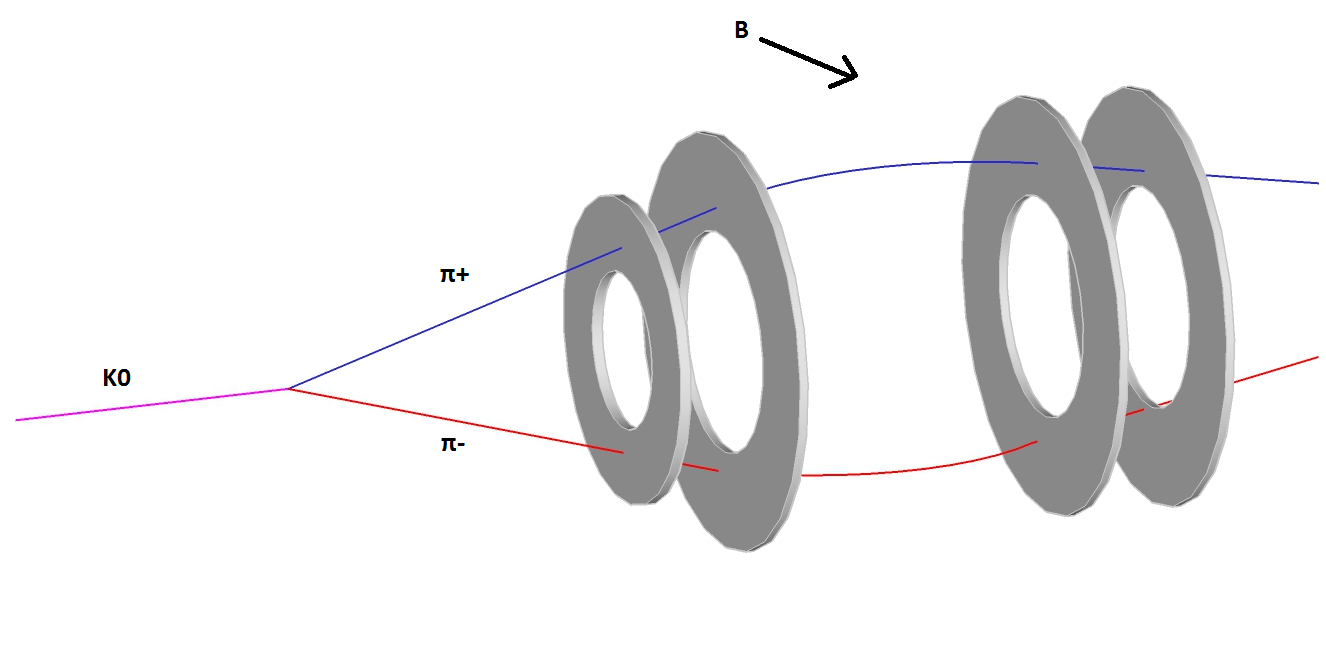
\includegraphics[scale=0.4]{apparato_3d} 
		\caption{Riproduzione 3D dell'apparato sperimentale: con $\vec{B}$ è indicato il vettore del campo magnetico, nella direzione positiva delle $x$.}
		\label{fig:apparato_3d}
	\end{center}
\end{figure}

\begin{figure}
	\begin{center}
		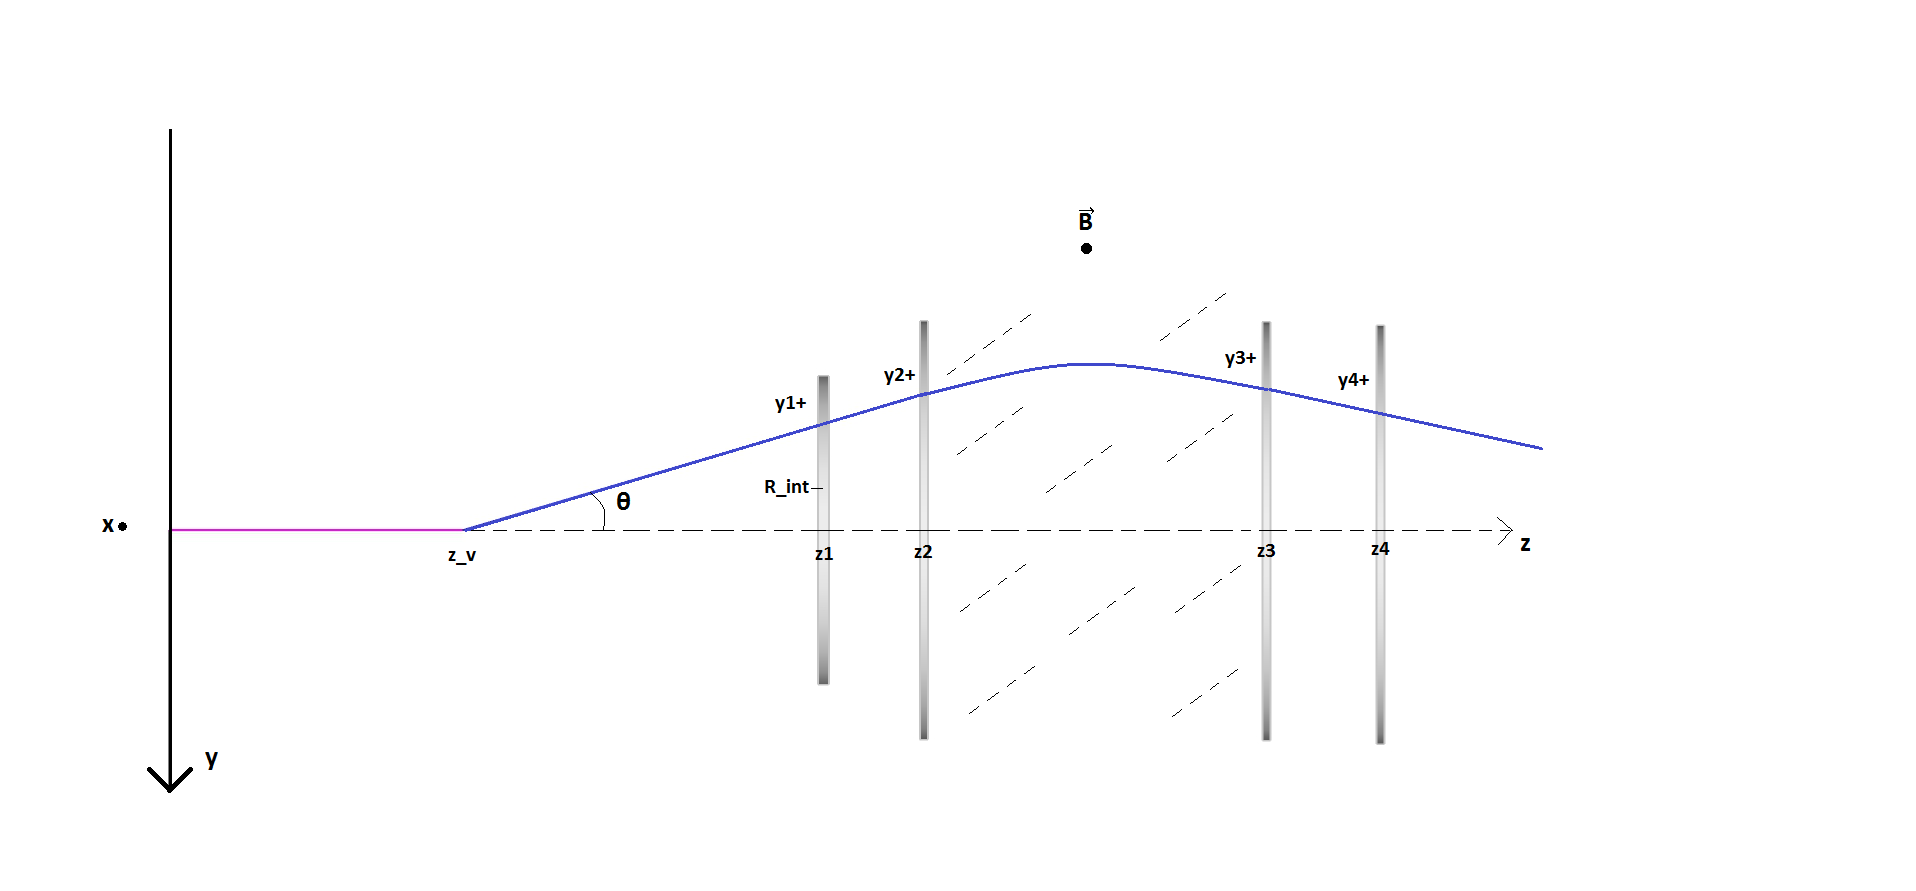
\includegraphics[scale=0.4]{apparato_2d}
		\caption{Sezione dell'apparato sperimentale: in viola lungo l'asse z, la traccia del $K^0$ genitore, in blu e rosso rispettivamente le tracce delle particelle decadute $\pi^+$ e $\pi^-$. Il campo magnetico, nella direzione positiva delle $x$, è uscente perpendicolarmente dal piano della figura. Con $z_i$ sono indicate le coordinate $z$ dei quattro piani di rivelatore. Con $R_{int}$, invece, il raggio interno del rivelatore più vicino.}
		\label{fig:apparato_2d}
	\end{center}
\end{figure}

Ogni piano di rivelatore è modellizzato da una corona circolare di raggio interno $R_{int}$ e raggio esterno $R_{ext}$, con risoluzione fissa sugli assi $x$ e $y$ di $1\ mm$\footnote{Come si vedrà in Sez.\ref{sec:detector}, la risposta del rivelatore è assunta gaussiana e la risoluzione indicata è dunque uguale alla deviazione standard di questa distribuzione.}. Sebbene quest'ultimo sia importante a livello pratico nel disegno del rivelatore, ai fini di questa simulazione questo sarà sempre considerabile infinito, poiché scelto in modo tale da contenere l'interezza dei decadimenti. La scelta del raggio interno è invece soggetta a differenti necessità, che saranno discusse più avanti (Sez. \ref{subsec:raggio_interno}!!!!!!!!!!!!. Il campo magnetico è situato in una zona di $0.35\ m$ al centro tra i piani $2$ e $3$, che distano tra loro $3\ m$ e vale $B = 1\ T$. Il $p_{kick}$ corrispondente vale quindi circa $p_k = qB\Delta L = 105\ MeV/c$. La modellizzazione dell'effetto di un magnete come un kick effettuato nel punto medio tra i rivelatori sarà giustificata in sez.\ref{sec:generation} !!!!!!!!!!. In Tab.\ref{tab:apparato} sono riassunte le caratteristiche scelte per l'apparato e la lunghezza media di decadimento, con $\mathbf{<\lambda>} = \frac{<p>}{M_{K}} c \tau$, $\tau = 8.954 \cdot 10^{-11} \ s$.

\bigskip

\begin{table} [h!]
\centering
\begin{tabular}{||p {1.5 cm}|p {1 cm}||}
\hline \hline
$\mathbf{{<\lambda>}(m)}$ & 5.4 \\ 
\hline
$\mathbf{z_1(m)}$ & 50 \\ 
\hline
$\mathbf{z_2(m)}$ & 60 \\ 
\hline
$\mathbf{z_3(m)}$ & 63 \\ 
\hline
$\mathbf{z_4(m)}$ & 73 \\
\hline
$\mathbf{R_{int}(m)}$ & 0.1 \\
\hline
$\mathbf{p_k}(MeV/c)$ & 105 \\
\hline
$\mathbf{B}(T)$ & 1 \\
\hline
$\mathbf{\Delta L}(m)$ & 0.35 \\
\hline
$\mathbf{\sigma_x}(m)$ & 0.001 \\
\hline \hline
\end{tabular} 
\caption{Tabella riassuntiva delle caratteristiche dell'apparato sperimentale.}
\label{tab:apparato}
\end{table}





\end{document}